\section{Cấu trúc cây thư mục của mã nguồn}
Việc cần làm đầu tiên và quan trọng nhất là tổ chức files và các thư mục. Với một thiết kế tốt thì khi làm việc chung giữa nhiều người sẽ ít bị đụng độ. Nhóm lựa chọn cách chia mỗi thành phần của trang ra từng module tách biệt với nhau, thuận lợi cho việc mở rộng và bảo trì, bảo dưỡng.\\

Dựa vào kiến trúc hệ thống mà nhóm đã thiết kế ở trên, nhóm đã thiết kế cấu trúc mã nguồn như sau:
\begin{center}
  \captionsetup{type=figure}
  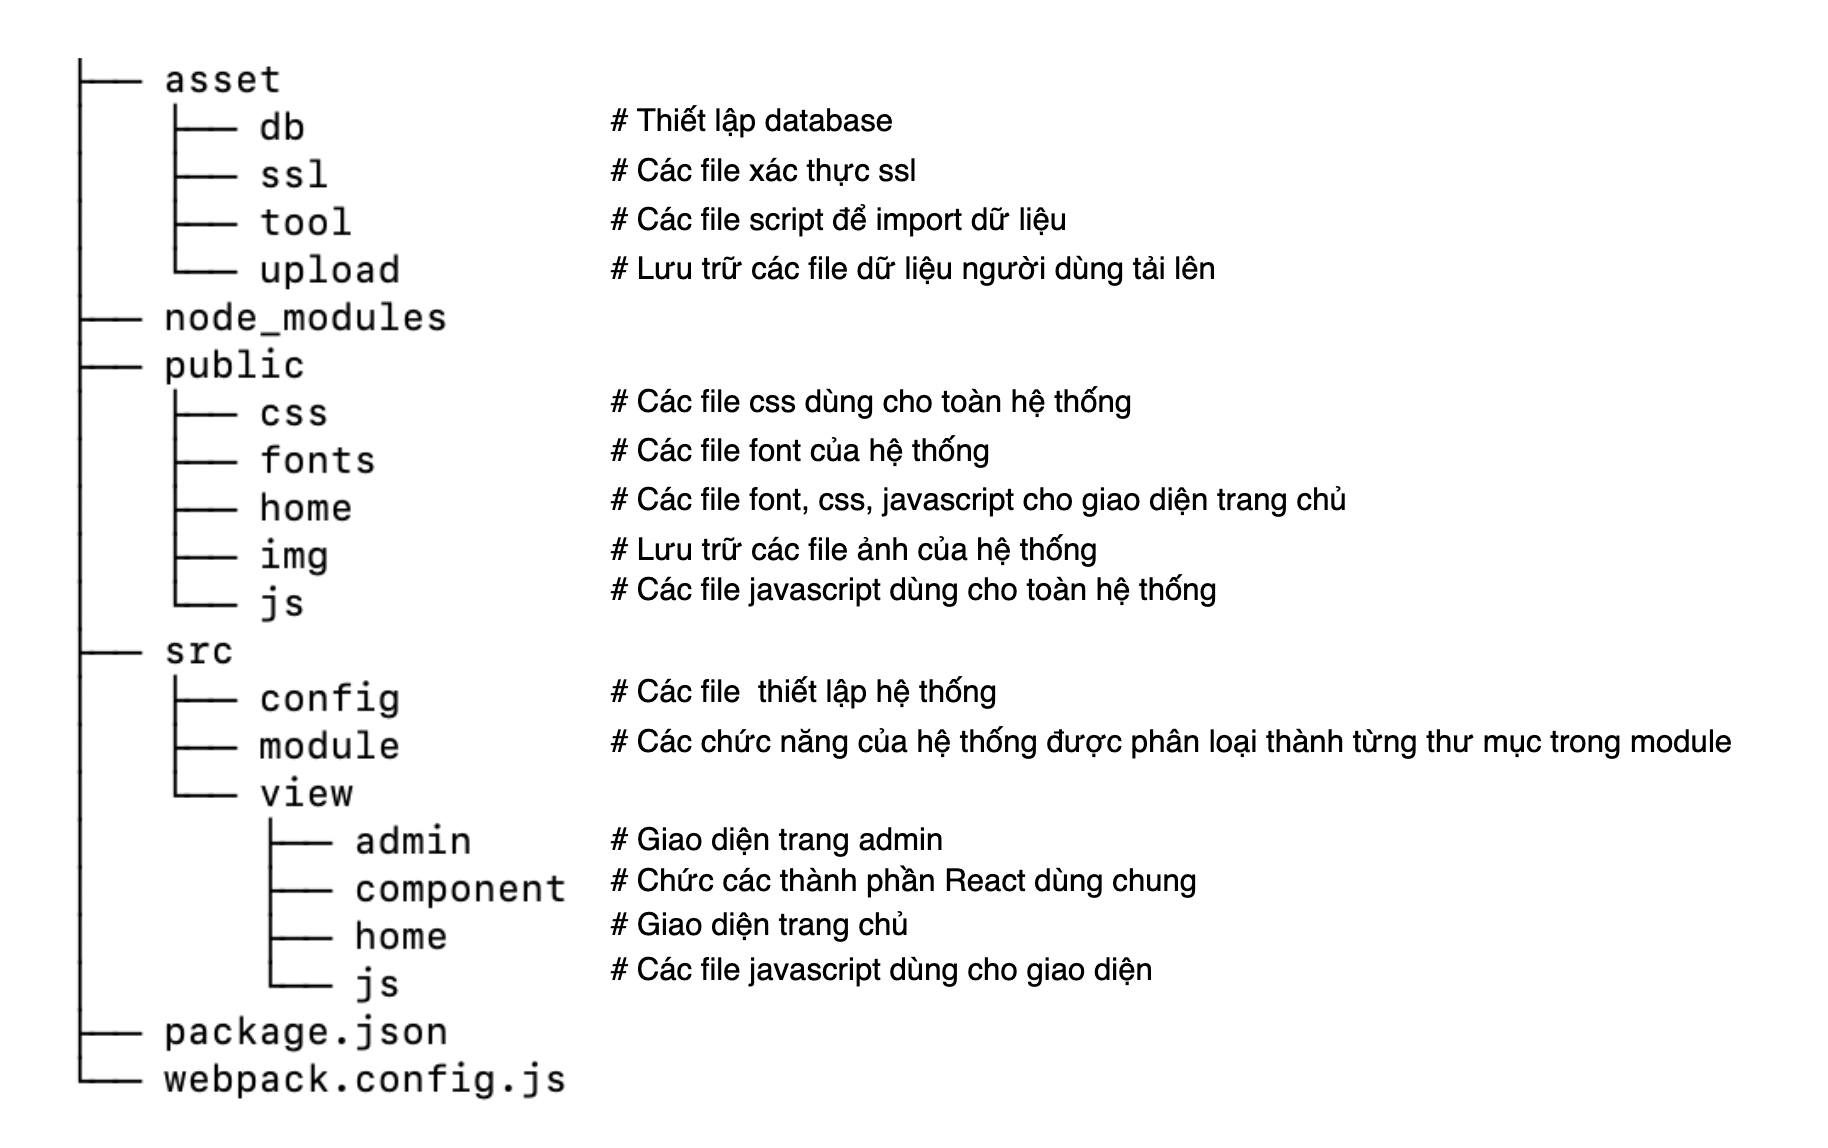
\includegraphics[width=15cm]{img/tree.png}
  \captionof{figure}{Cây thư mục của hệ thống}
\end{center}

Nhóm chia các danh mục, quá trình, chức năng vào từng module riêng, các module được thiết kế thống nhất theo mô hình MVC kết hợp với Redux. 

Cách chia module này thuận lợi cho phân chia công việc, tránh đụng độ trong phát triển hệ thống, dễ dàng thêm các module mới trong quá trình mở rộng, giúp cho việc tìm và sửa lỗi trong quá trình bảo trì trở nên đơn giản hơn.

\begin{figure}[H]
    \centering
    \begin{subfigure}[b]{0.4\linewidth}
        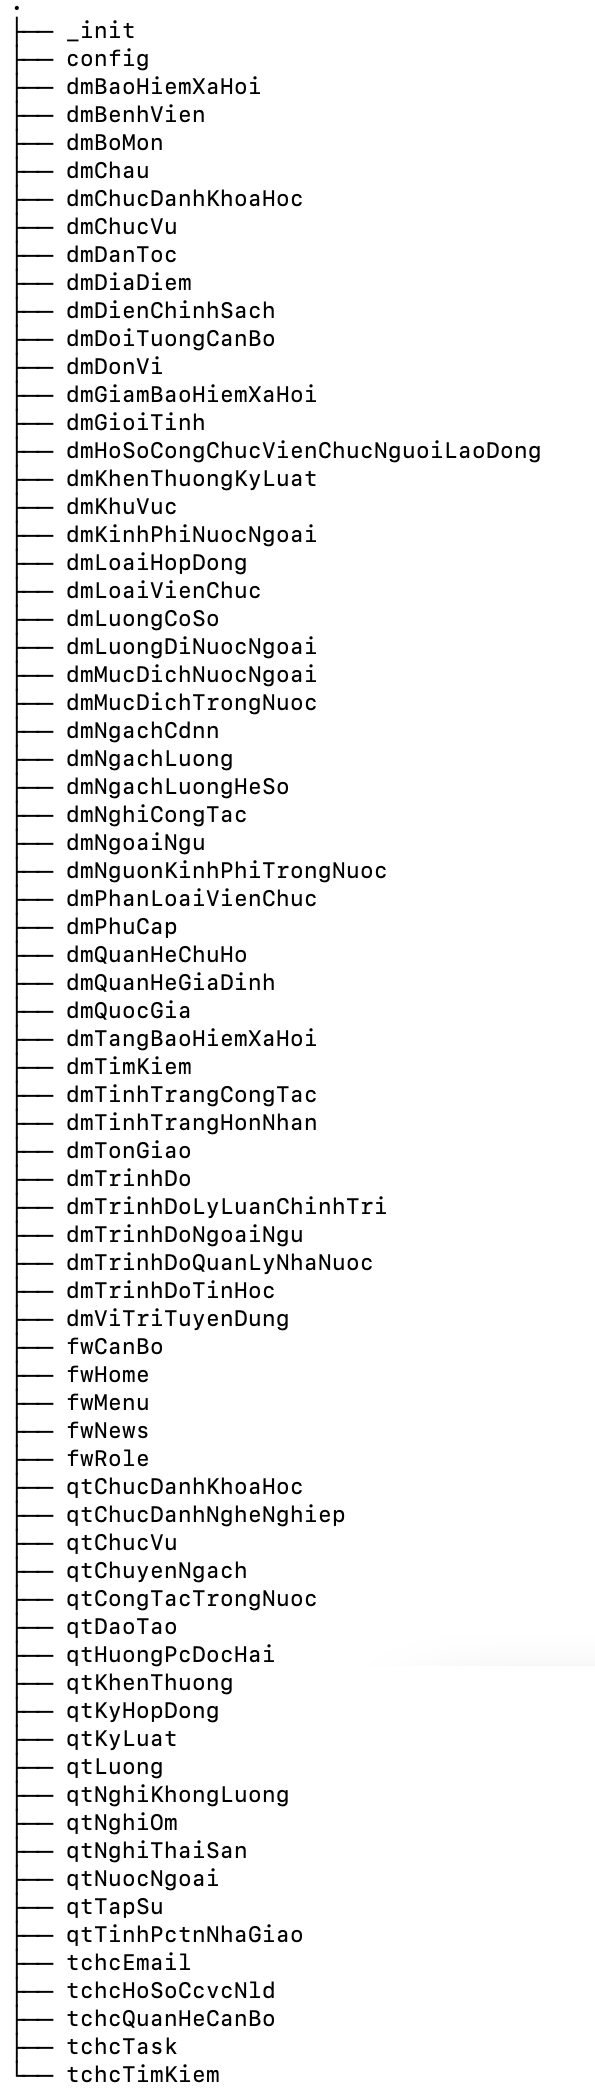
\includegraphics[width=\linewidth]{img/module.png}
        \caption{Thư mục module}
    \end{subfigure}
    \begin{subfigure}[b]{0.4\linewidth}
        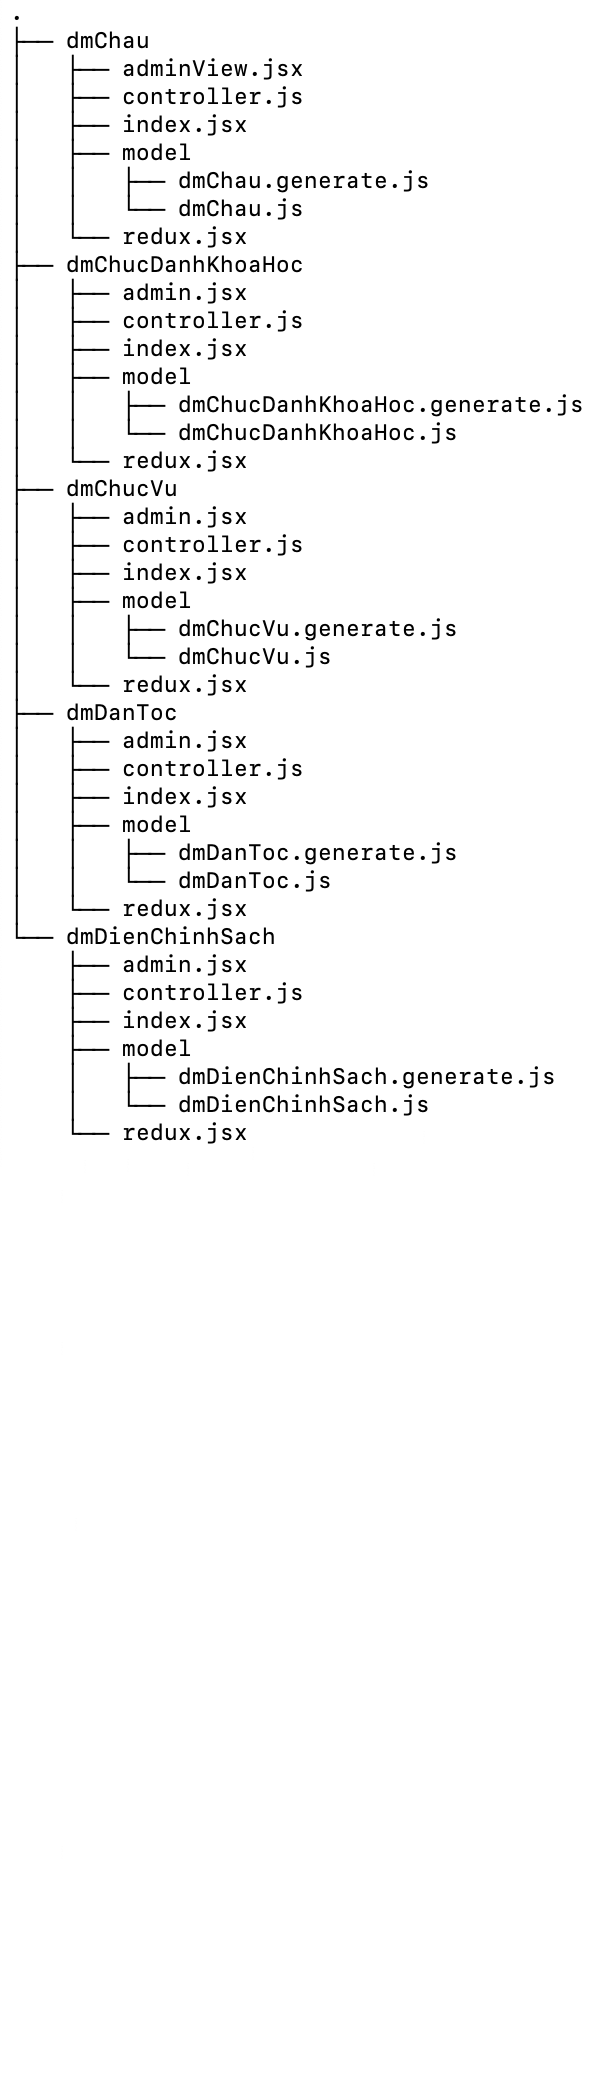
\includegraphics[width=\linewidth]{img/moduleDetail.png}
        \caption{Chi tiết từng module}
    \end{subfigure}
    \caption{Thư mục module của hệ thống}
\end{figure}
\section{Xác thực đối tượng người dùng}
Hệ thống xác thực đối tượng người dùng bằng hệ thống xác thực tập trung (SSO) của trường Đại học Bách Khoa - ĐHQG-HCM.
\begin{center}
  \captionsetup{type=figure}
  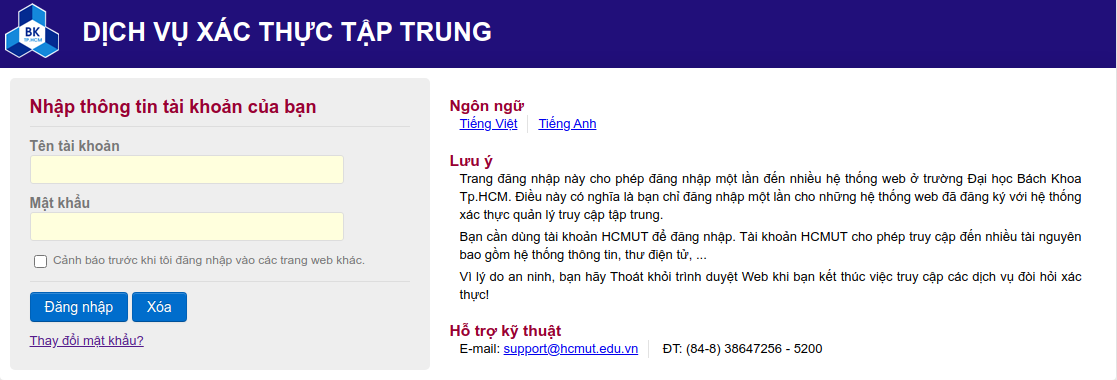
\includegraphics[width=15cm]{img/Screen/sso.png}
  \captionof{figure}{Hệ thống xác thực tập trung}
\end{center}

Người dùng sử dụng tài khoản trường Đại học Bách Khoa của mình để đăng nhập. Sau khi đăng nhập thành công, hệ thống xác thực tập trung (SSO) sẽ trả về cho hệ thống email tài khoản của người dùng. Lúc này hệ thống sẽ kiểm tra, email nhận được đã được quản trị viên thêm vào hệ thống thì người dùng sẽ đăng nhập được vào hệ thống và thực hiện các chức năng với vai trò của mình.\\

Đối với từng vai trò, sau khi đăng nhập vào hệ thống sẽ có các menu như sau:
\begin{center}
  \captionsetup{type=figure}
  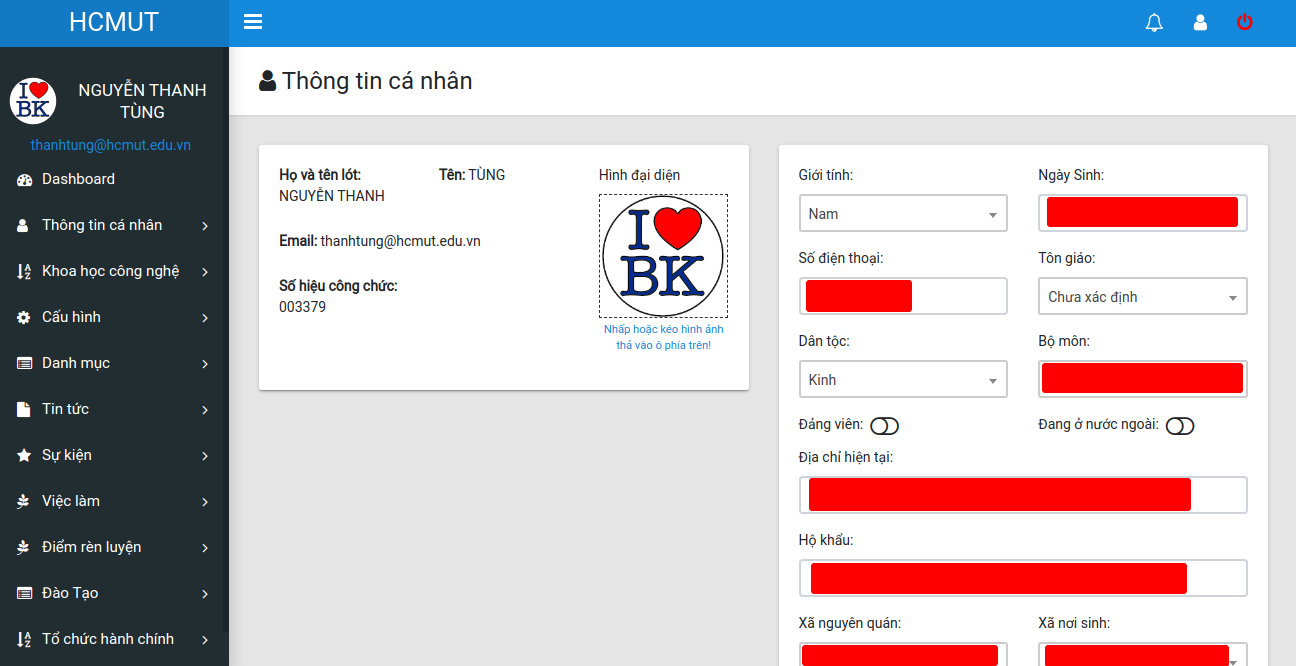
\includegraphics[width=15cm]{img/Screen/admin.png}
  \captionof{figure}{Menu của người dùng là quản trị hệ thống}
\end{center}
\begin{center}
  \captionsetup{type=figure}
  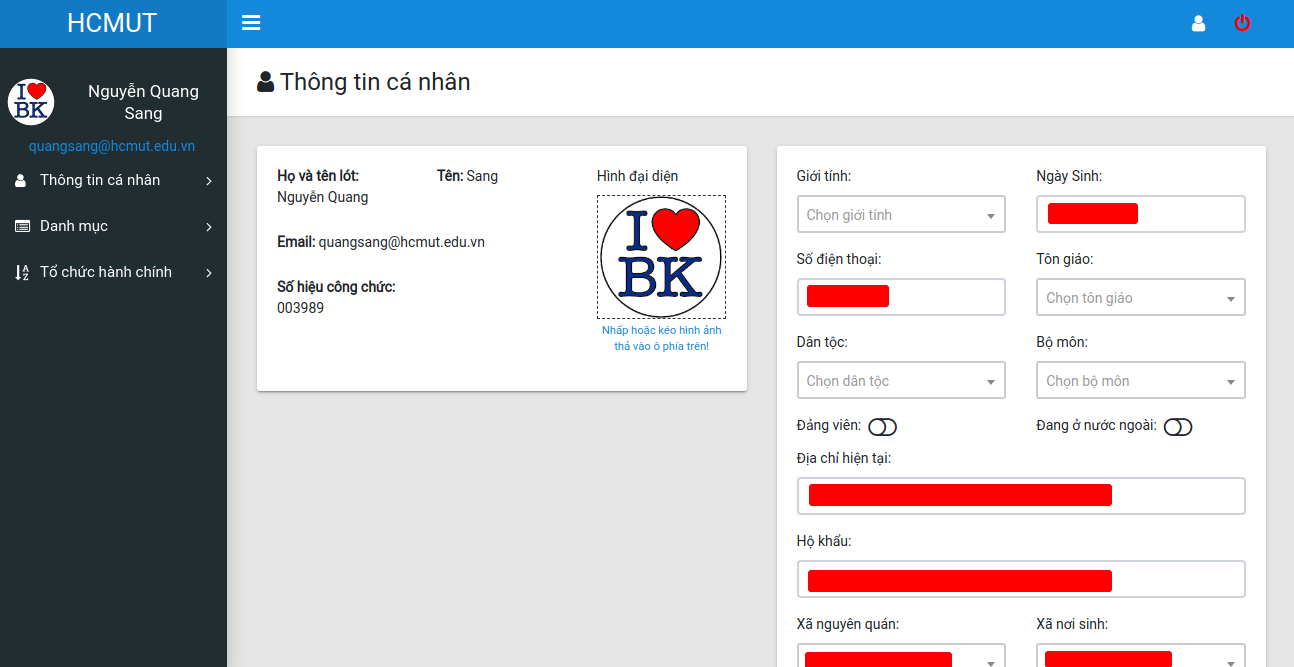
\includegraphics[width=15cm]{img/Screen/manager.png}
  \captionof{figure}{Menu của người dùng là quản lý và cán bộ phòng Tổ chức - Hành chính}
\end{center}
\begin{center}
  \captionsetup{type=figure}
  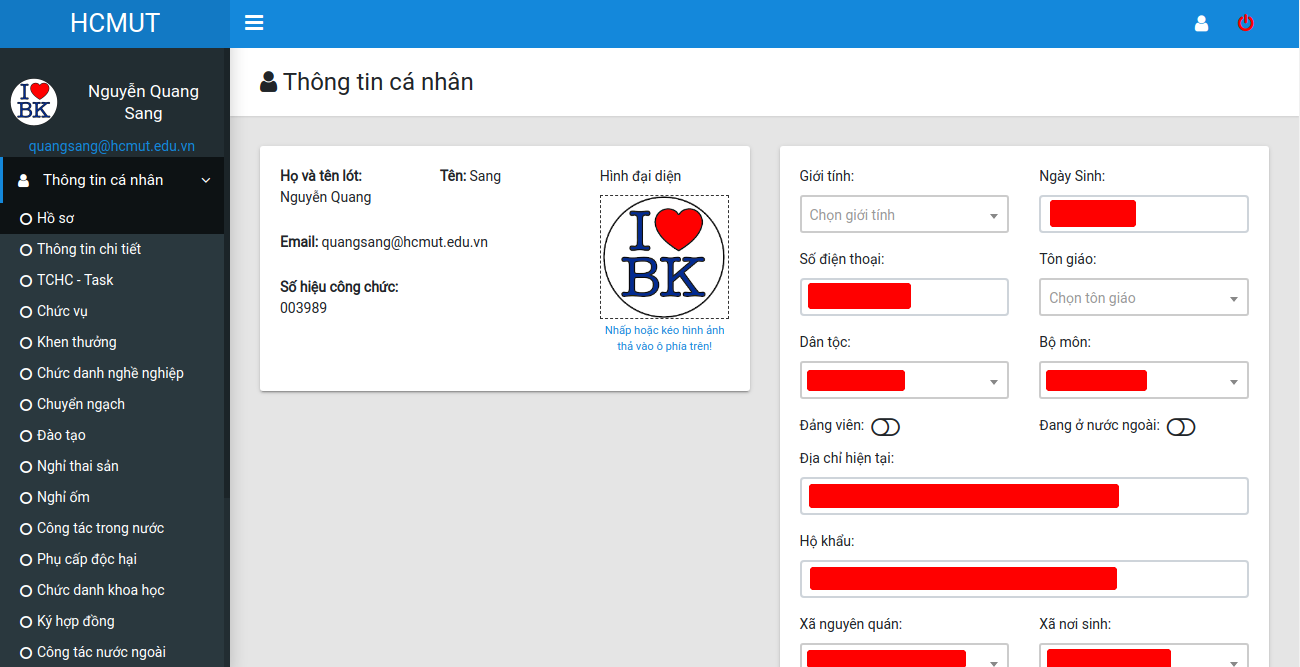
\includegraphics[width=15cm]{img/Screen/canbo.png}
  \captionof{figure}{Menu của người dùng là CBCNV của trường}
\end{center}
\section{Chức năng từng đối tượng trong hệ thống}
Từ việc thiết kế Usecase ở chương 4, nhóm nghiên cứu tiến hành thực hiện từng chức năng tương ứng với mỗi đối tượng. Cụ thể từng chức năng quan trọng như sau:
\subsection{Đối tượng: Quản trị hệ thống}
\subsubsection{Chức năng: Quản lý tài khoản người dùng}
 \begin{center}
  \captionsetup{type=figure}
  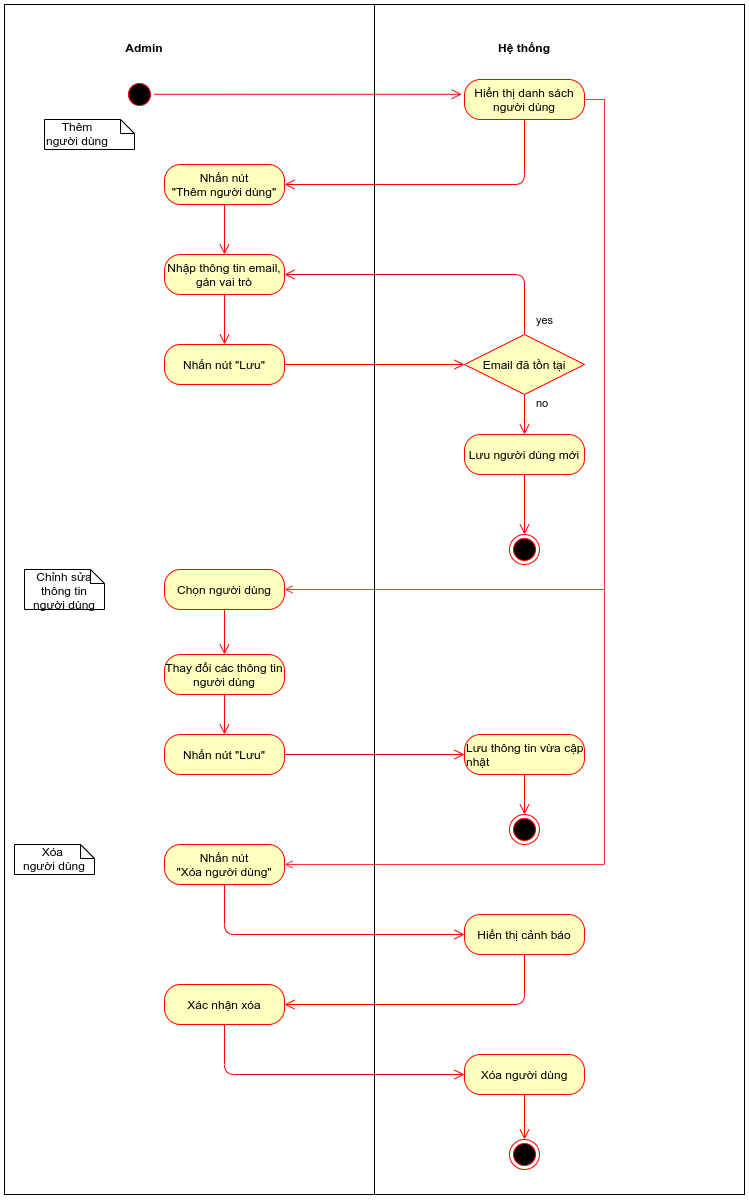
\includegraphics[width=12cm]{img/UML/Admin/UserMgt.png}
  \captionof{figure}{Lược đồ Activity quản lý tài khoản người dùng}
\end{center}
\begin{figure}[H]
    \centering
    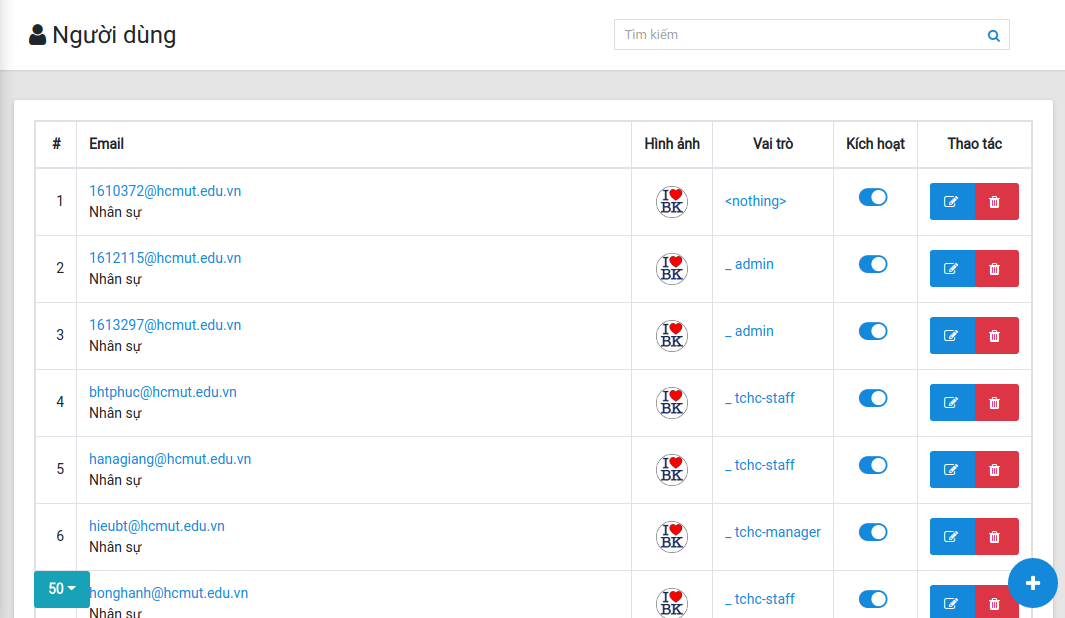
\includegraphics[width=15cm]{img/Screen/user.png}
    \caption{Danh sách người dùng hiện có của hệ thống}
    \label{fig:fig_danh_sach_nguoi_dung}
\end{figure}
Phần này giúp quản trị viên quản lý được người dùng trong hệ thống. Quản trị viên có xem danh toàn bộ người dùng (hình \ref{fig:fig_danh_sach_nguoi_dung}); chỉnh sửa các thông tin của từng người dùng, đặt vai trò trong hệ thống, kích hoạt tài khoản (hình \ref{fig:fig_edit_nguoi_dung}), xóa người dùng khỏi hệ thổng.\\
\begin{figure}[H]
    \centering
    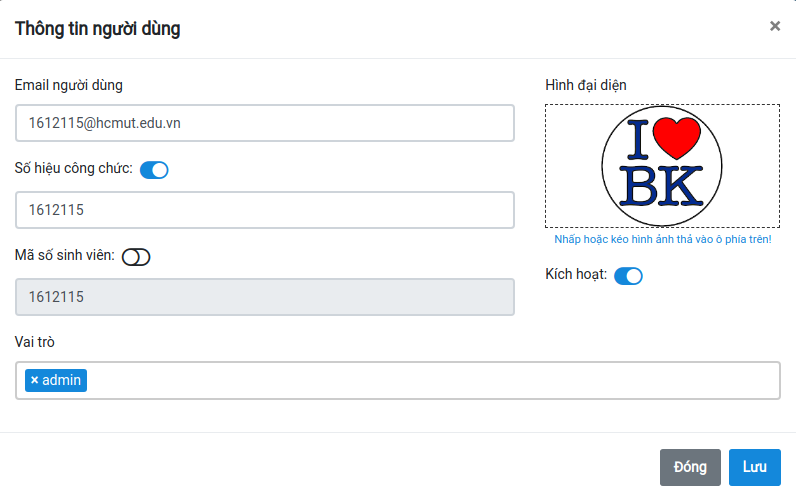
\includegraphics[width=15cm]{img/Screen/editUser.png}
    \caption{Chỉnh sửa thông tin người dùng}
    \label{fig:fig_edit_nguoi_dung}
\end{figure}
\subsubsection{Chức năng: Quản lý vai trò trong hệ thống}
\begin{center}
  \captionsetup{type=figure}
  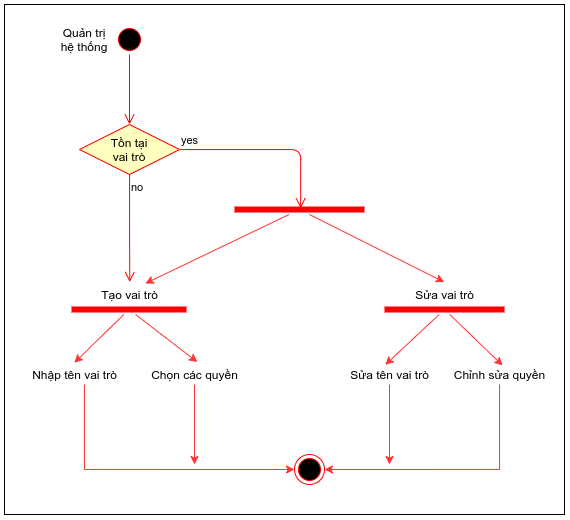
\includegraphics[width=15cm]{img/UML/Admin/addRole.png}
  \captionof{figure}{Lược đồ Activity quản lý vai trò hệ thống}
\end{center}

Hệ thống tồn tại cơ chế quản lý vai trò động. Mỗi vai trò được gán với các quyền truy cập. Quản trị viên có thể chỉnh sửa quyền của các vai trò một cách dễ dàng.\\
\begin{center}
  \captionsetup{type=figure}
  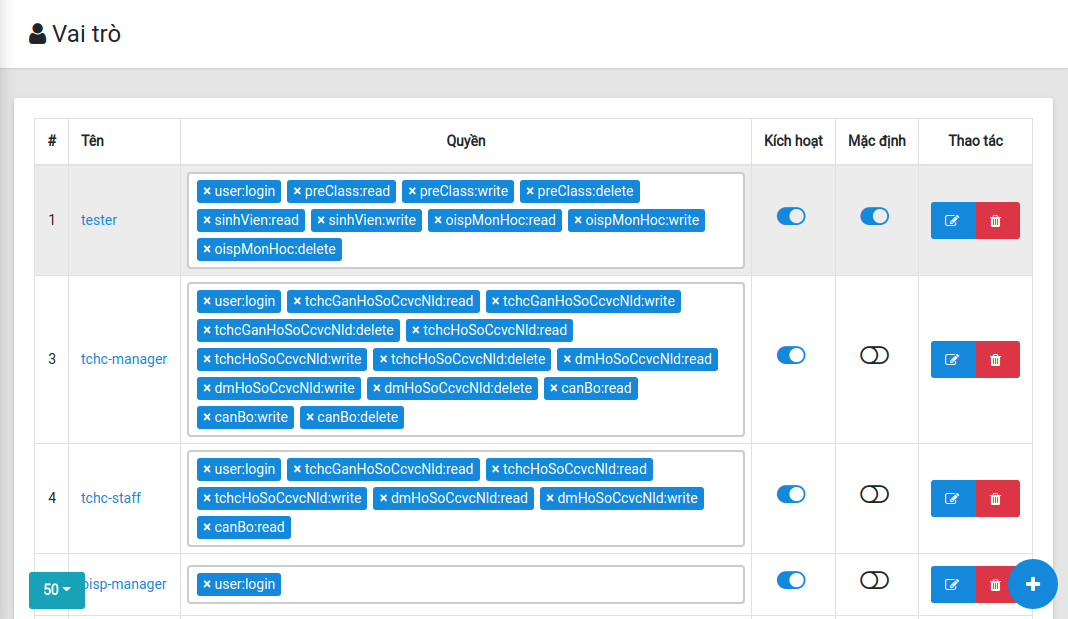
\includegraphics[width=15cm]{img/Screen/allrole.png}
  \captionof{figure}{Danh sách vai trò có trong hệ thống hiện tại}
\end{center}
\begin{center}
  \captionsetup{type=figure}
  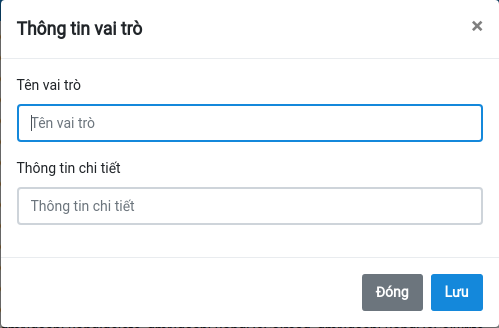
\includegraphics[width=15cm]{img/Screen/addrole.png}
  \captionof{figure}{Thêm một vai trò vào hệ thống}
\end{center}
\begin{center}
  \captionsetup{type=figure}
  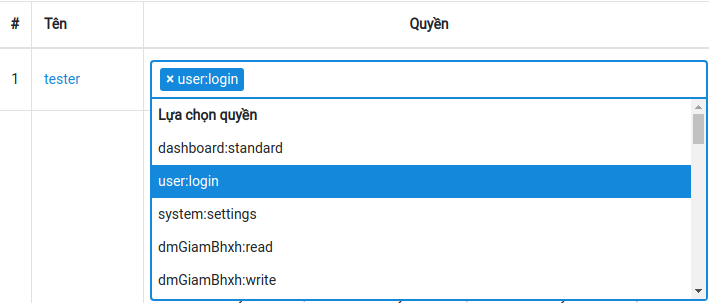
\includegraphics[width=15cm]{img/Screen/ganquyen.png}
  \captionof{figure}{Thay đổi các quyền cho vai trò}
\end{center}
\subsubsection{Chức năng: Quản lý trang chủ}
\textbf{Tạo, chỉnh sửa menu}
\begin{center}
  \captionsetup{type=figure}
  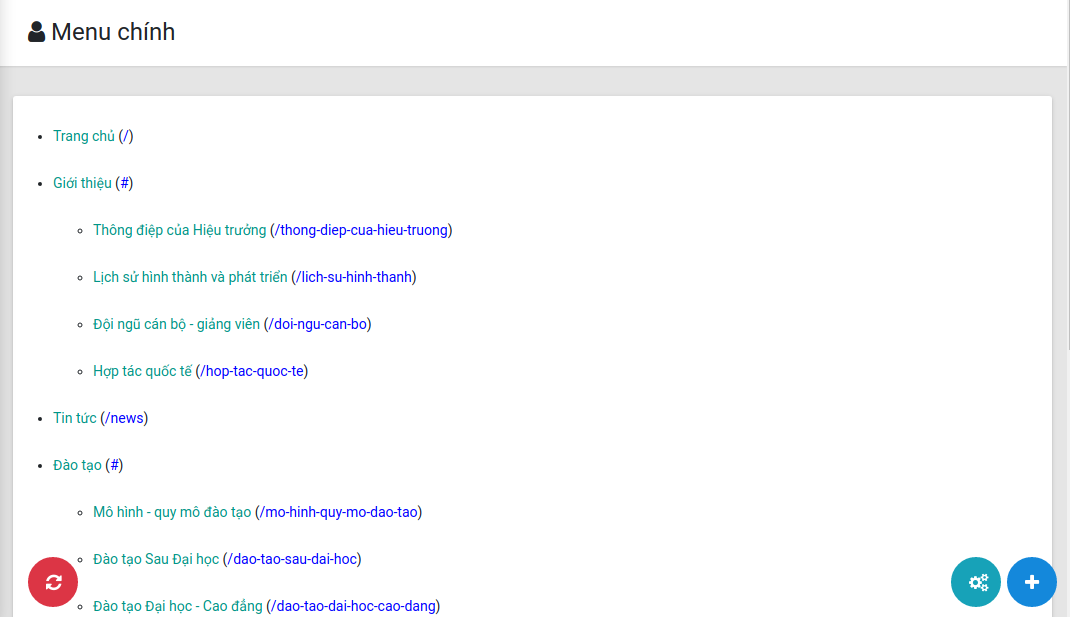
\includegraphics[width=15cm]{img/Screen/menu.png}
  \captionof{figure}{Danh sách menu của trang}
\end{center}

Phần này giúp quản trị viên thiết kế phần menu header của trang chủ như là: tạo mới menu kèm theo đường dẫn, tạo menu con, kích hoạt menu, thay đổi thứ tự hiển thị.\\

\textbf{Chức năng: Cấu hình các Section trong một trang giao diện cụ thể}
\begin{center}
  \captionsetup{type=figure}
  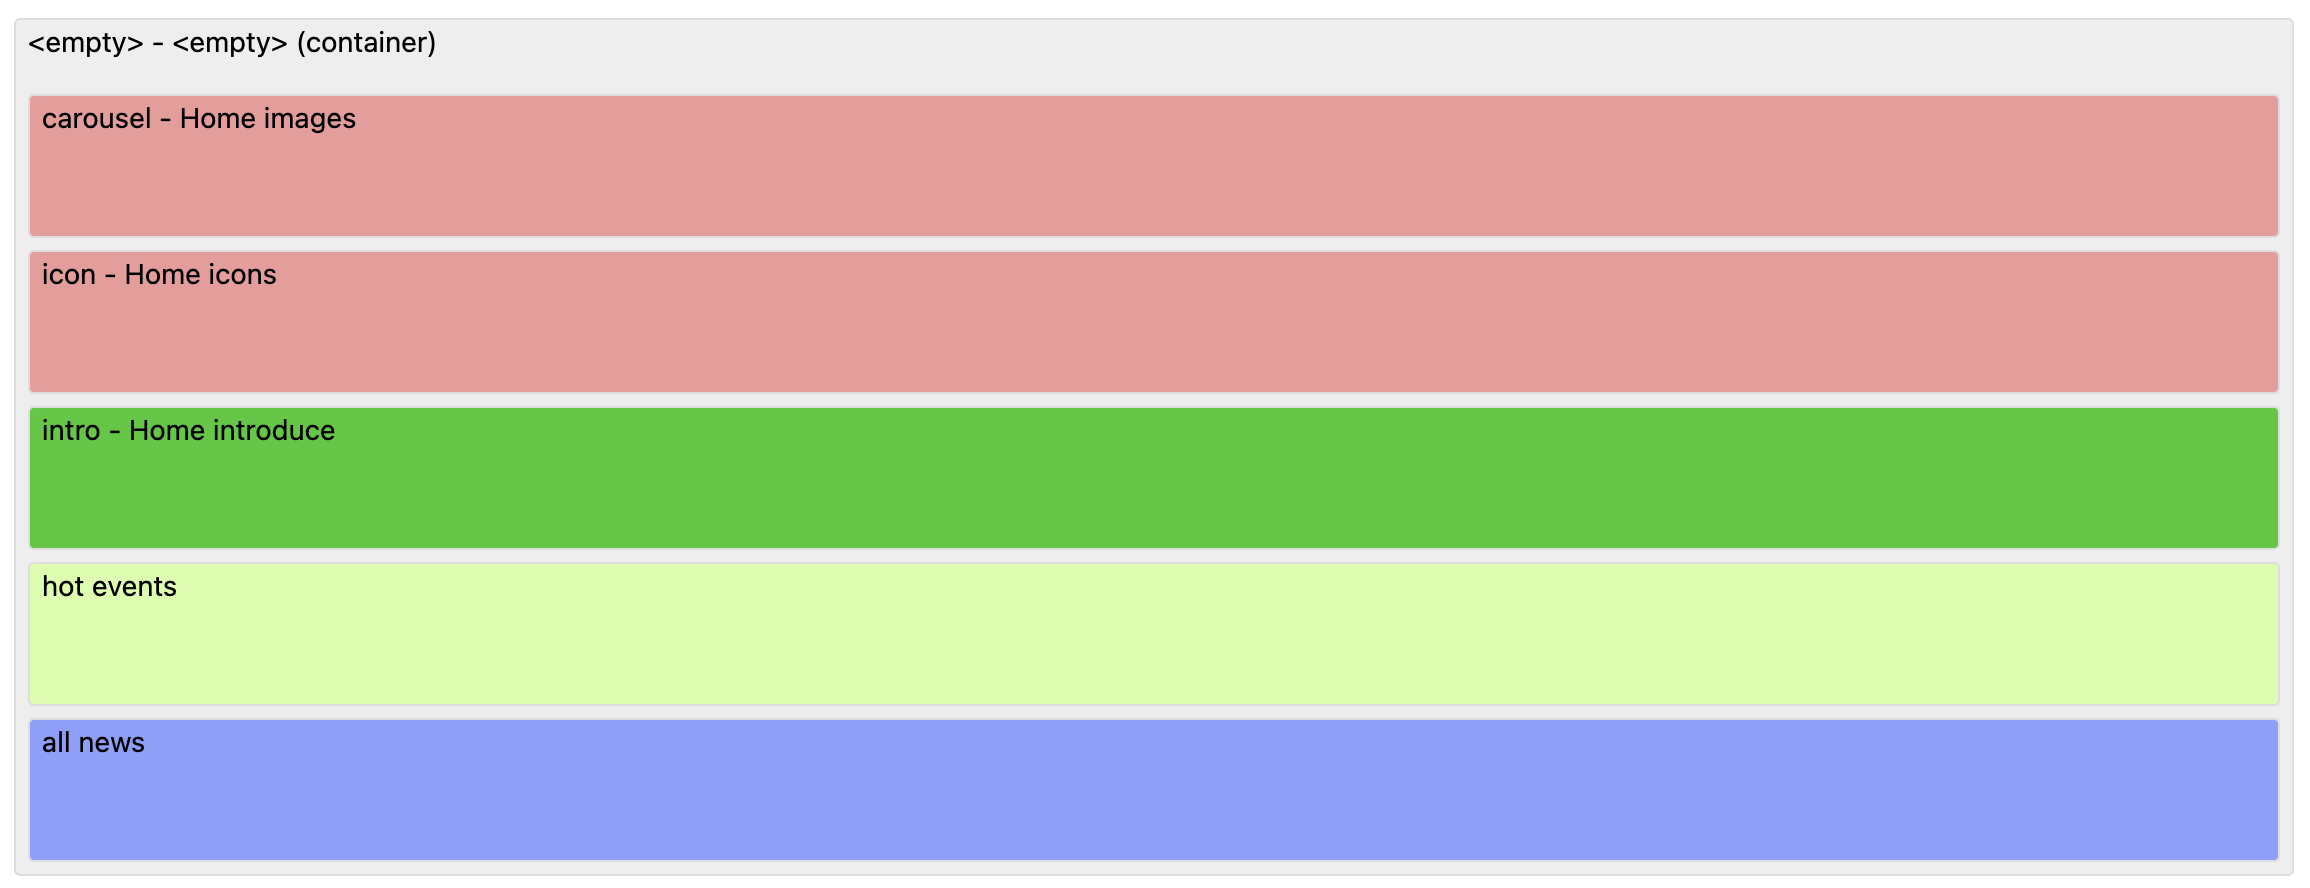
\includegraphics[width=15cm]{img/Screen/section.png}
  \captionof{figure}{Danh sách section của một trang giao diện cụ thể}
\end{center}

Ở một trang chủ cụ thể, quản trị viên có thể thiết lập trang đó gồm những thành phần nào và thứ tự xuất hiện của các thành phần đó.\\

\textbf{Chức năng: Quản lý thông tin danh mục}\\
\begin{center}
  \captionsetup{type=figure}
  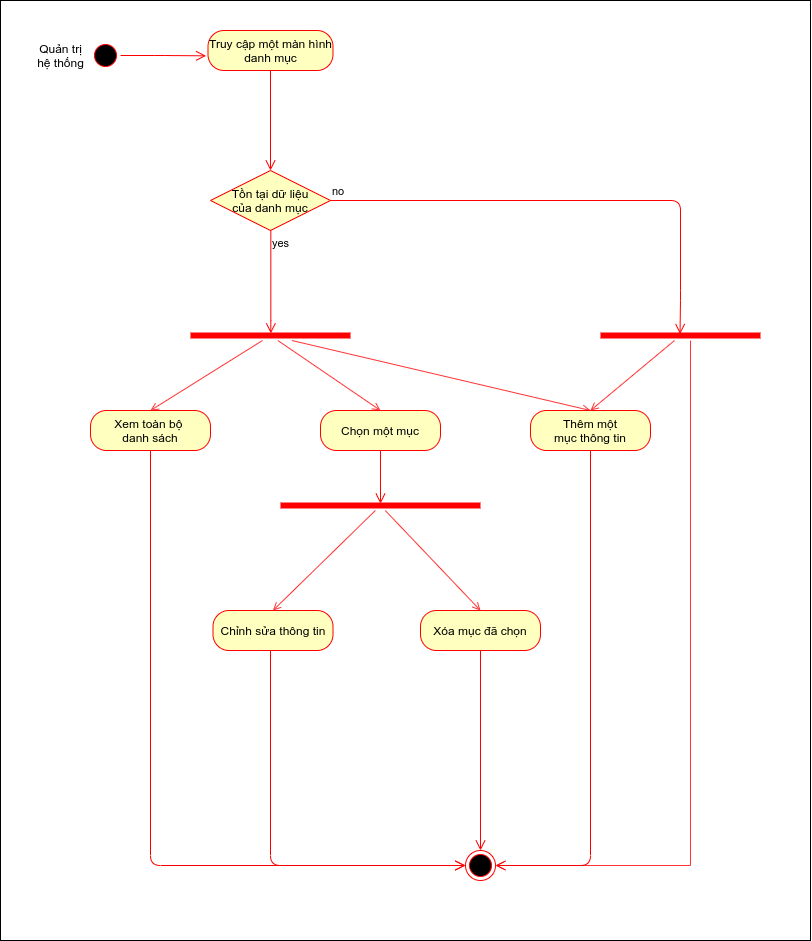
\includegraphics[width=15cm]{img/UML/Admin/danhmucActivity.png}
  \captionof{figure}{Lược đồ Activity quản lý danh mục}
\end{center}

Chức năng cho phép người quản trị hệ thống quy định các thông tin danh mục phục vụ cho việc nhập và lưu dữ liệu.\\
\begin{center}
  \captionsetup{type=figure}
  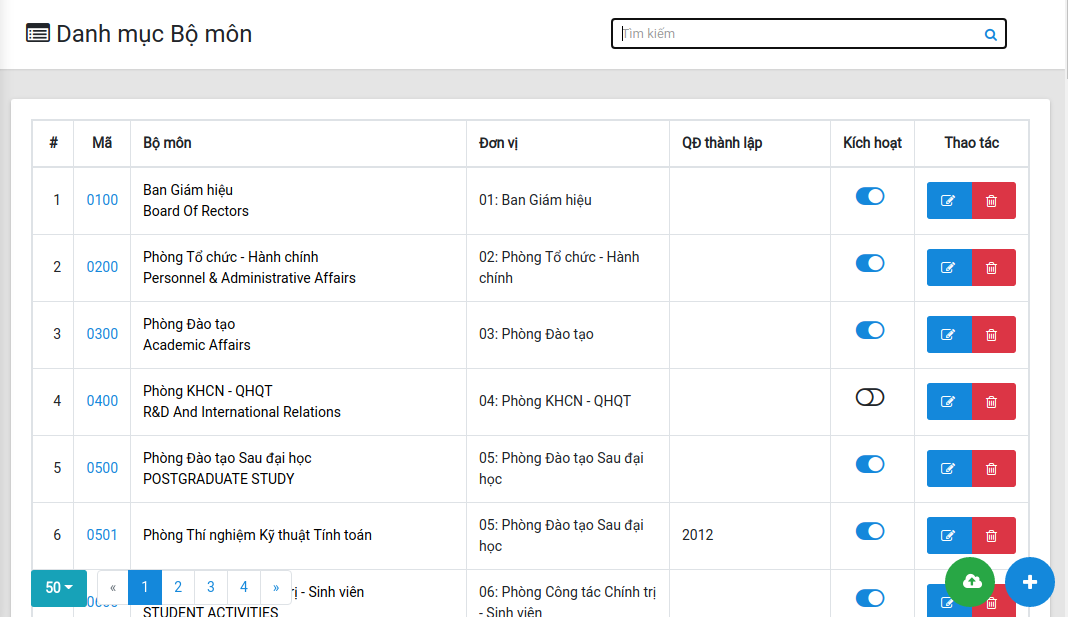
\includegraphics[width=15cm]{img/Screen/danhmuc.png}
  \captionof{figure}{Danh sách danh mục bộ môn}
\end{center}
\subsection{Đối tượng: Quản lý phòng Tổ chức - Hành chính}
\subsubsection{Chức năng: Quản lý nhân viên phòng Tổ chức - Hành chính}
\begin{center}
  \captionsetup{type=figure}
  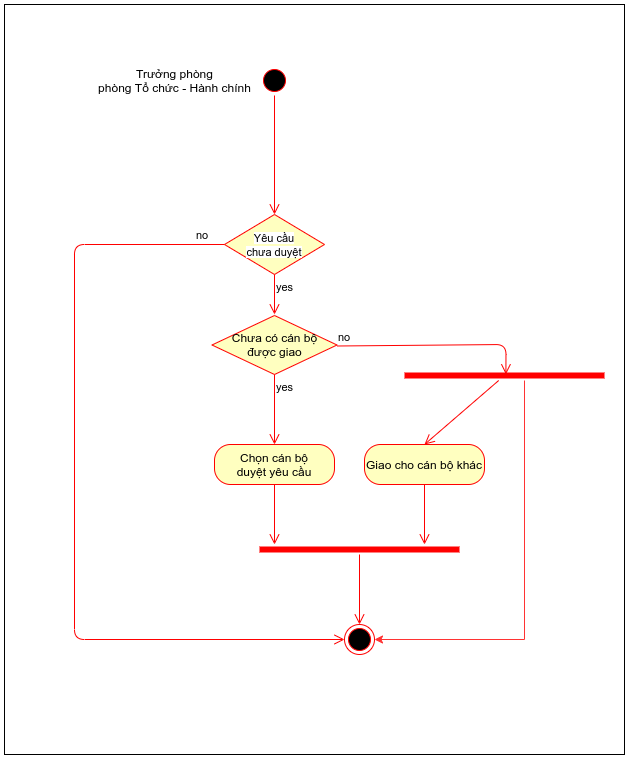
\includegraphics[width=15cm]{img/UML/Manager/assignTask.png}
  \captionof{figure}{Lược đồ Activity cho chức năng phân công cán bộ duyệt yêu cầu}
\end{center}
\begin{figure}[H]
    \centering
    \begin{subfigure}[b]{0.4\linewidth}
        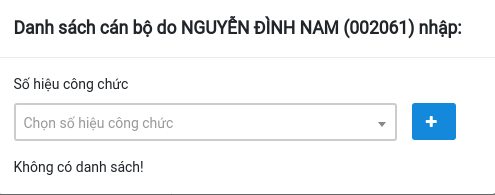
\includegraphics[width=\linewidth]{img/Screen/assignhoso.png}
        \caption{Phân công cán bộ nhập hồ sơ}
        \label{fig:assign_hoso}
    \end{subfigure}
    \begin{subfigure}[b]{0.4\linewidth}
        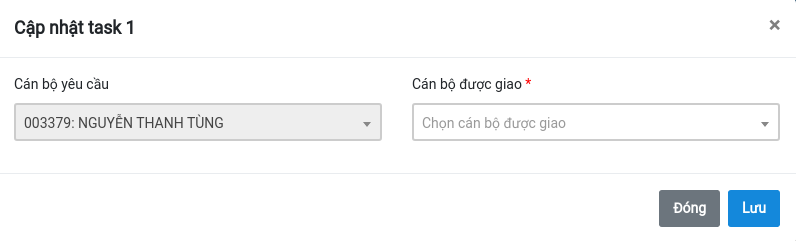
\includegraphics[width=\linewidth]{img/Screen/assignTask.png}
        \caption{Phân công cán bộ duyệt yêu cầu}
        \label{fig:assign_task}
    \end{subfigure}
    \caption{Phân công cho cán bộ phòng Tổ chức - Hành chính}
\end{figure}
\subsubsection{Chức năng cấu hình phòng Tổ chức - Hành chính}
\textbf{Cấu hình thông tin email cho phòng Tổ chức - Hành chính}
\begin{figure}[H]
    \centering
    \begin{subfigure}[b]{0.4\linewidth}
        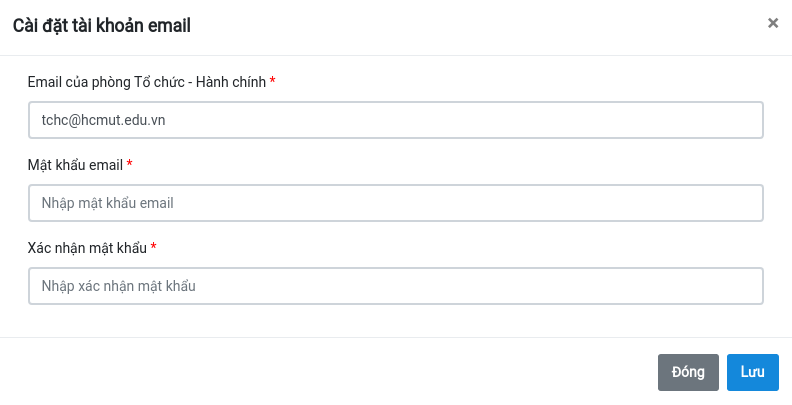
\includegraphics[width=\linewidth]{img/Screen/emailsetting.png}
        \caption{Cấu hình địa chỉ email}
        \label{fig:email_setting}
    \end{subfigure}
    \begin{subfigure}[b]{0.4\linewidth}
        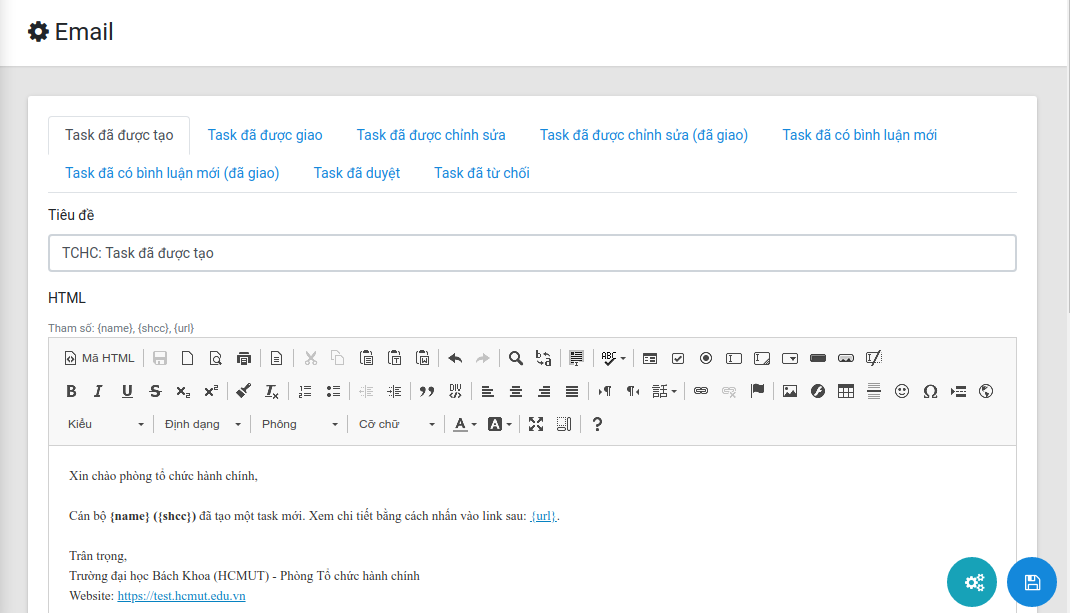
\includegraphics[width=\linewidth]{img/Screen/email.png}
        \caption{Cấu hình nội dung các email}
        \label{fig:email}
    \end{subfigure}
    \caption{Cấu hình email cho phòng Tổ chức - Hành chính}
\end{figure}

Phần này giúp quản trị viên thực hiện việc \textbf{soạn thảo nội dung} của email và nội dung của email này sẽ được sử dụng để thông báo cho những người dùng liên quan khi có các hoạt động liên quan đến yêu cầu. Trong nội dung của email, hệ thống có cung cấp những \textbf{tham số} được sử dụng khi cần thiết. Các tham số này sẽ được thay thế bằng những từ phù hợp bởi hệ thống trước khi gửi đi cho người dùng.\\

Ngoài ra, người quản lý phòng Tổ chức - Hành chính còn quản lý các danh mục liên quan đến phòng Tổ chức - Hành chính.
\subsubsection{Chức năng: Xem những thống kê của hệ thống}
\begin{center}
  \captionsetup{type=figure}
  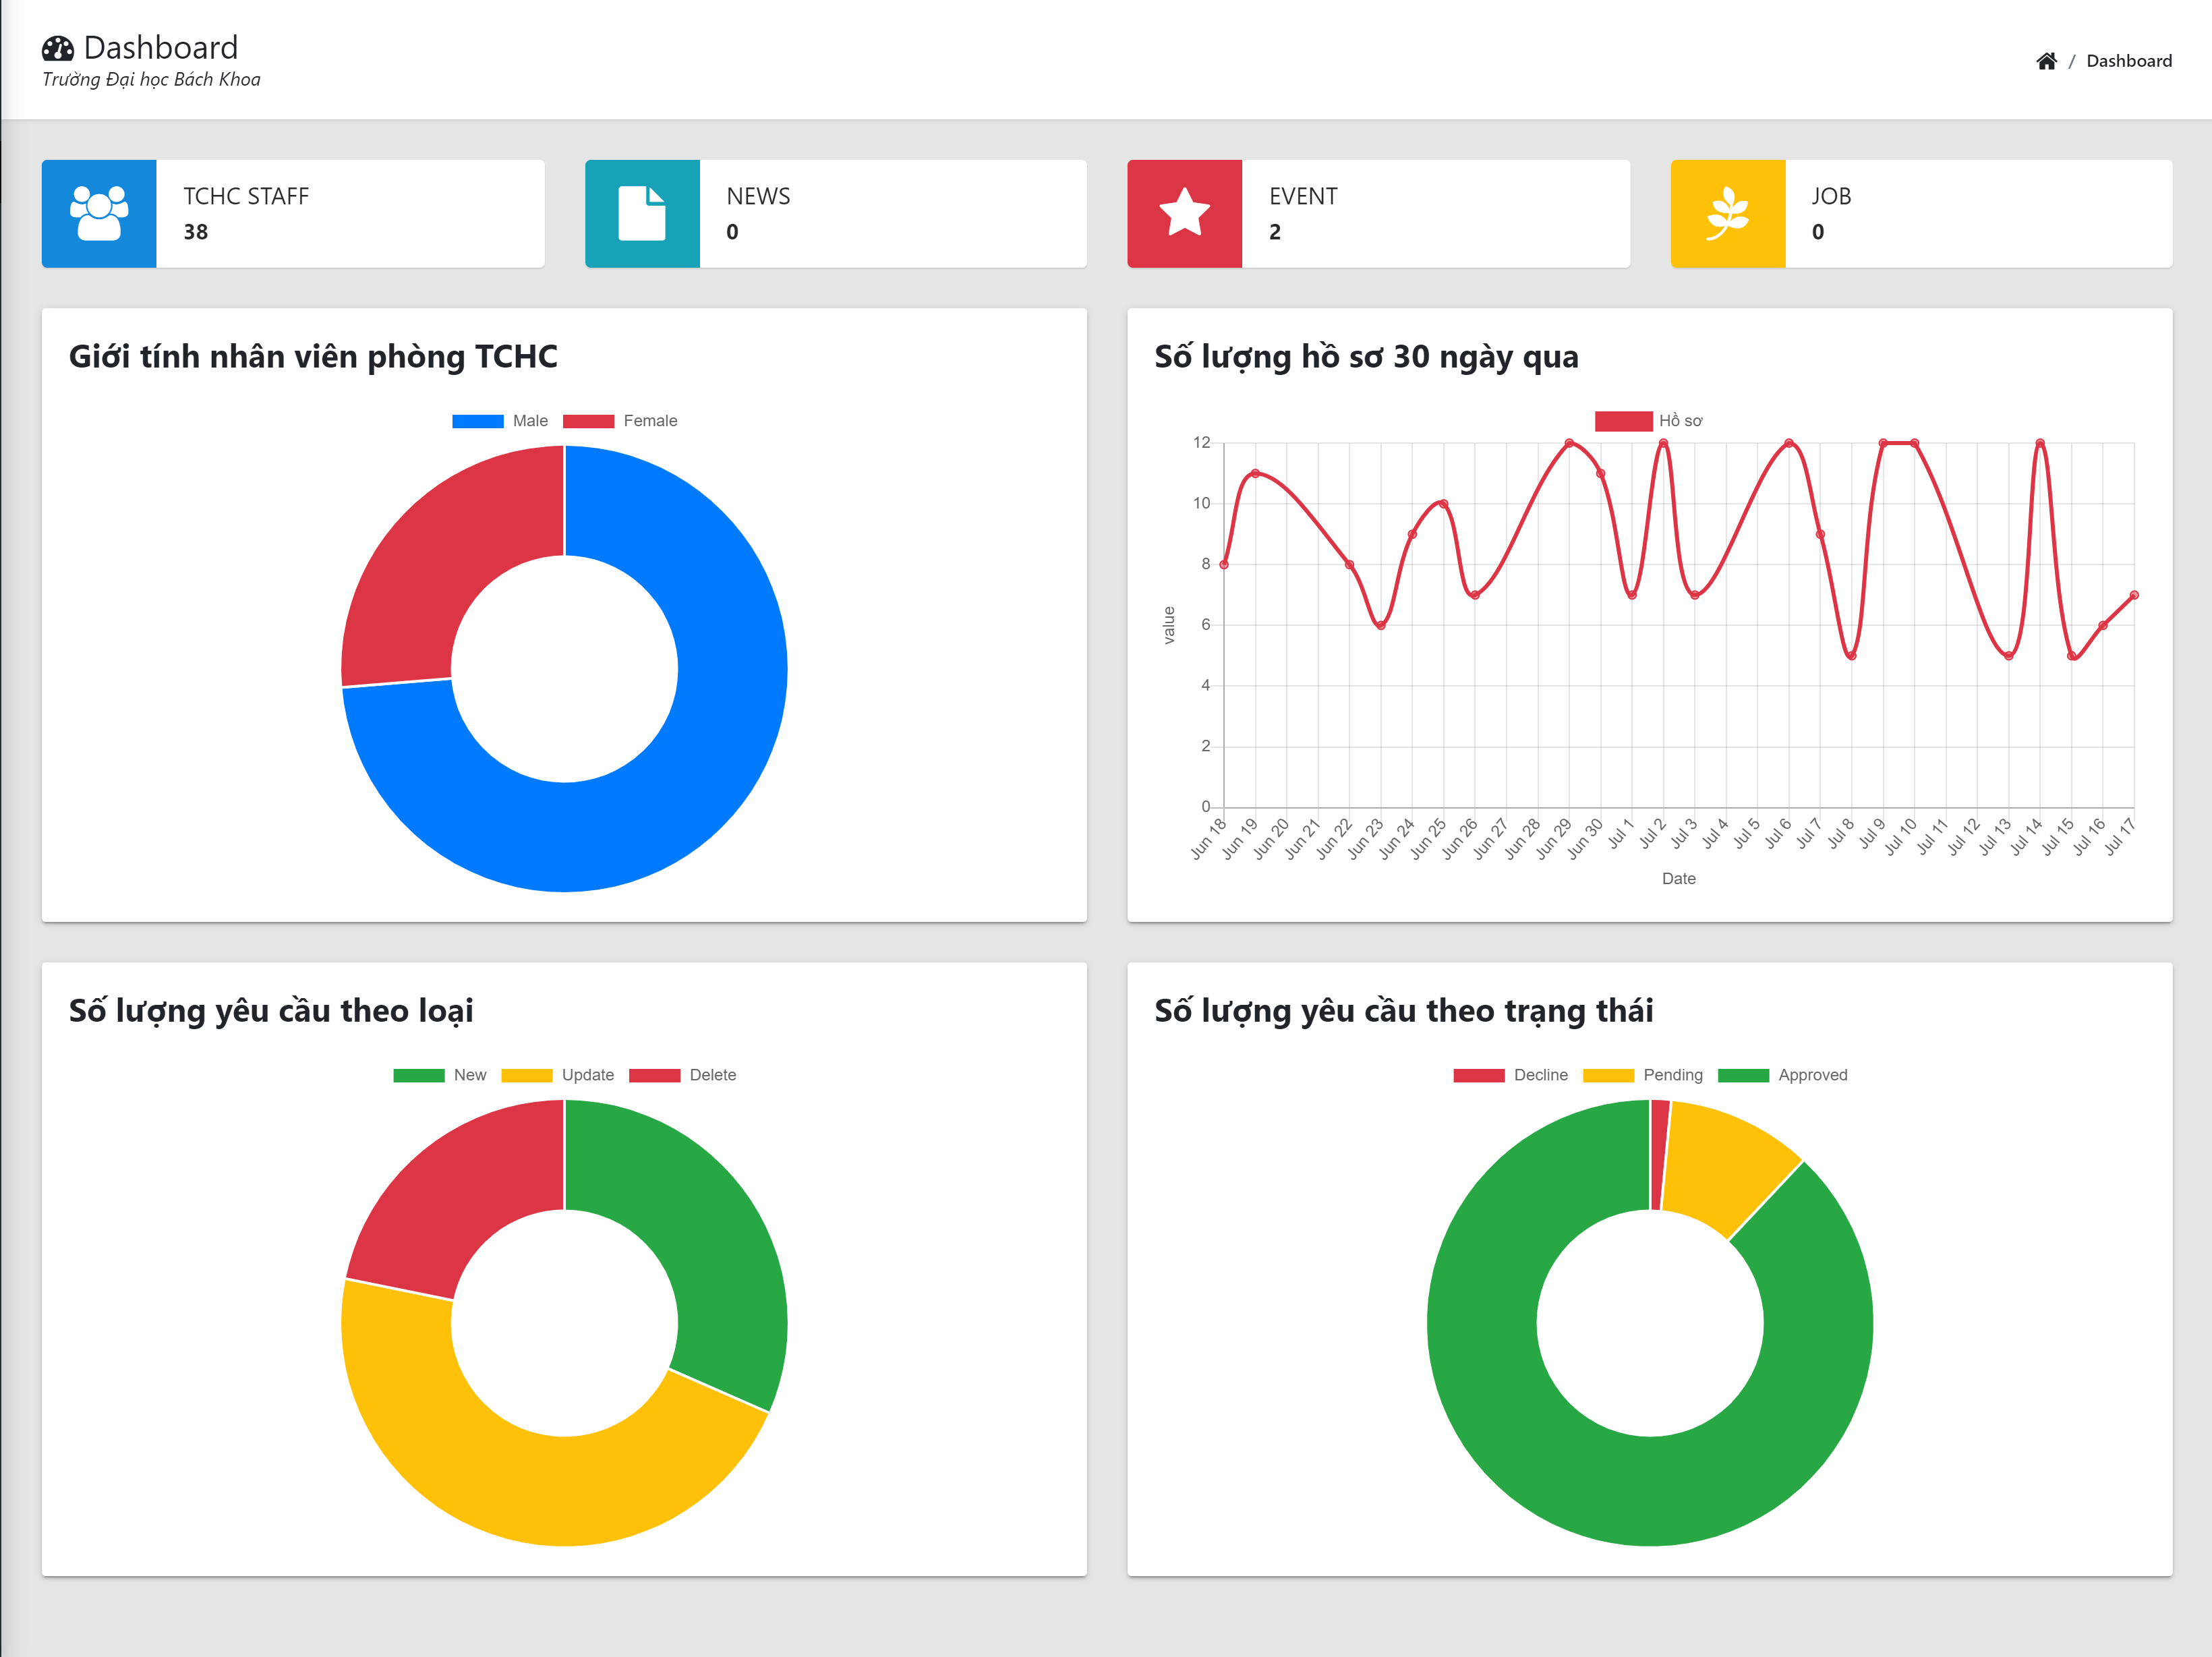
\includegraphics[width=15cm]{img/UML/User/dashboard.png}
  \captionof{figure}{Xem thống kê}
\end{center}

Quản lý phòng Tổ chức - Hành chính có thể theo dõi những thống kê trong hệ thống dưới dạng biểu đồ trực quan, sinh động. Thống kê về một số dữ liệu như:
\begin{itemize}
    \item Số nhân viên phòng Tổ chức - Hành chính
    \item Số lượng hồ sơ được nhận trong tháng
    \item Tỉ lệ yêu cầu phân chia theo loại
    \item Tỉ lệ yêu cầu phân chia theo trạng thái
    \item Tỉ lệ giới tính của cán bộ
    \item Tỉ lệ giới tính của cán bộ theo 13 khoa
    \item Số lượng cán bộ đang công tác trong nước
    \item Số lượng cán bộ đang công tác nước ngoài
    \item Số lượng, tỉ lệ sinh viên theo các khoá
\end{itemize}
\subsection{Đối tượng: Cán bộ phòng Tổ chức - Hành chính}
\subsubsection{Chức năng: Gán hồ sơ công chức, viên chức cho cán bộ}
\begin{center}
  \captionsetup{type=figure}
  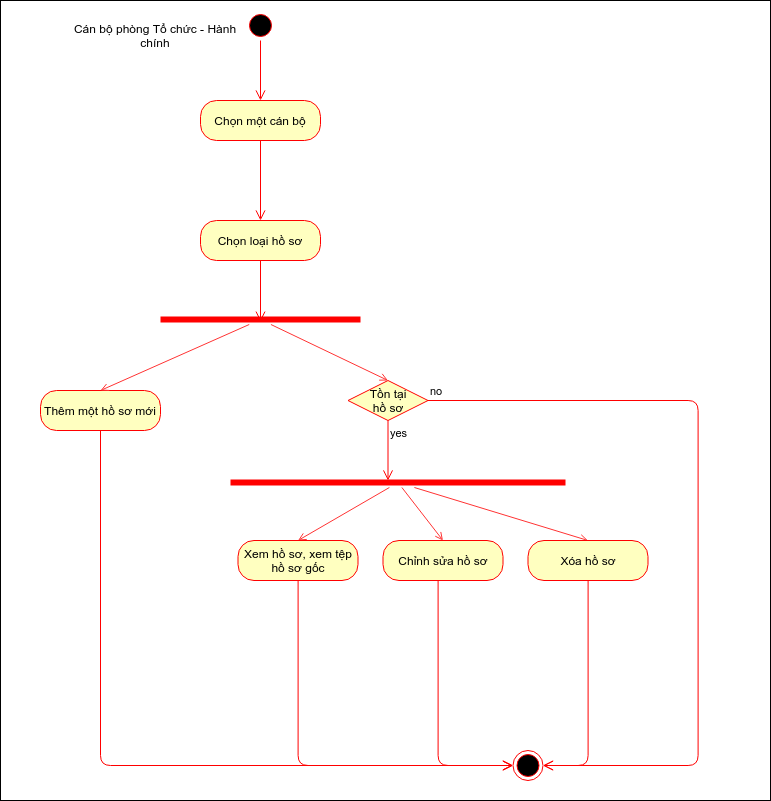
\includegraphics[width=15cm]{img/UML/TchcStaff/activityQuanLyHoSo.png}
  \captionof{figure}{Lược đồ Activity quản lý hồ sơ cán bộ}
\end{center}

Chức năng cho phép quản lý các hồ sơ của cán bộ. Lưu trữ hồ sơ gốc dưới dạng tệp trên hệ thống.
\begin{center}
  \captionsetup{type=figure}
  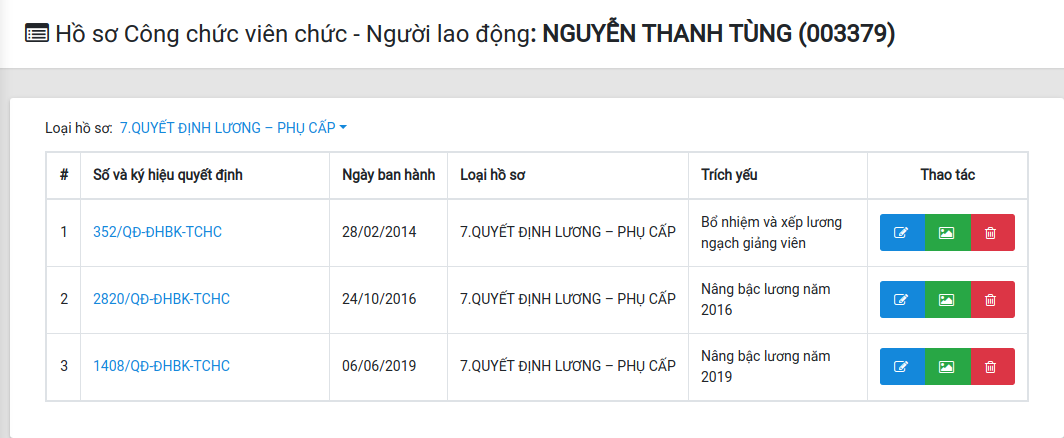
\includegraphics[width=15cm]{img/Screen/qlhoso.png}
  \captionof{figure}{Quản lý hồ sơ cán của một cán bộ}
\end{center}
\textbf{Chức năng: Quản lý cán bộ}\\
\begin{center}
  \captionsetup{type=figure}
  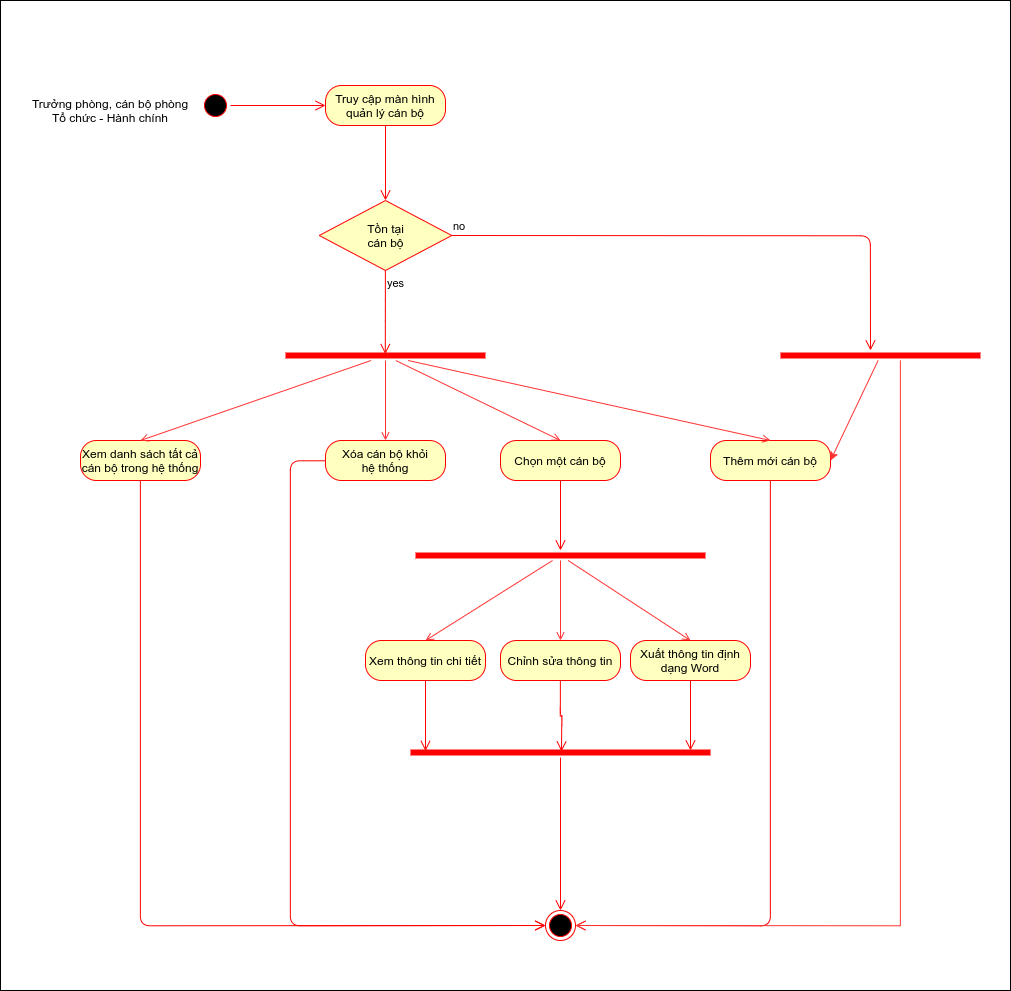
\includegraphics[width=15cm]{img/UML/TchcStaff/activityQuanLyCanBo.png}
  \captionof{figure}{Lược đồ Activity chức năng quản lý thông tin cán bộ}
\end{center}

Đây là chức năng cho phép đối tượng là cán bộ phòng Tổ chức - Hành chính có thể xem và chỉnh sửa thông tin của toàn bộ cán bộ hiện có trong hệ thống, thêm cán bộ vào hệ thống, xóa cán bộ khỏi hệ thống. Bên cạnh đó họ còn có thể xuất thông tin của cán bộ ra tệp tin Word theo mẫu của Bộ nội vụ.\\
\begin{center}
  \captionsetup{type=figure}
  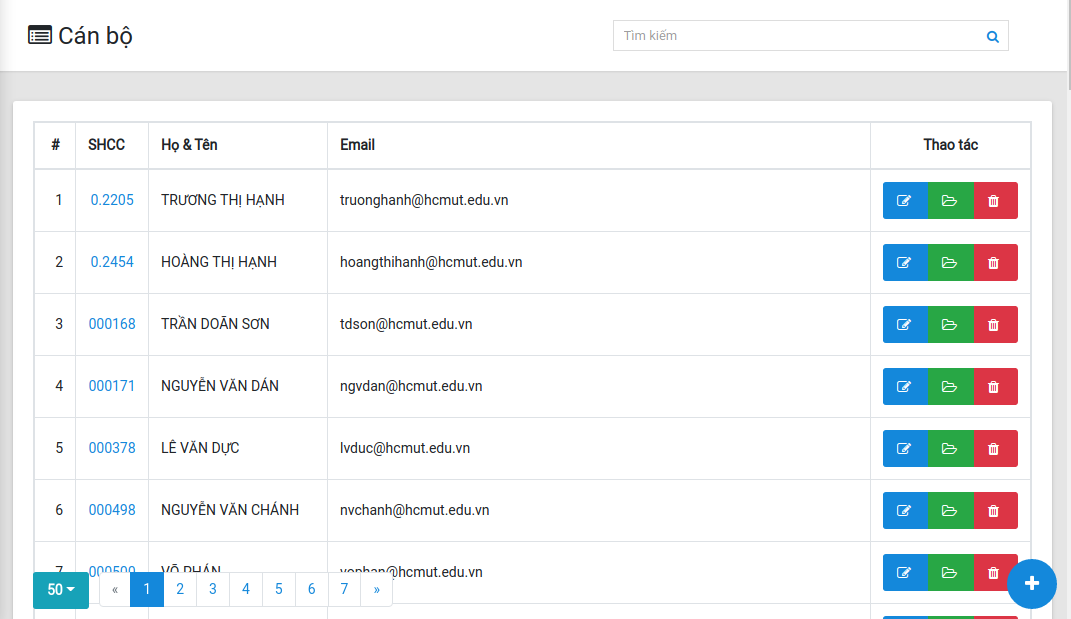
\includegraphics[width=15cm]{img/Screen/allcanbo.png}
  \captionof{figure}{Danh sách toàn bộ cán bộ}
\end{center}
\begin{center}
  \captionsetup{type=figure}
  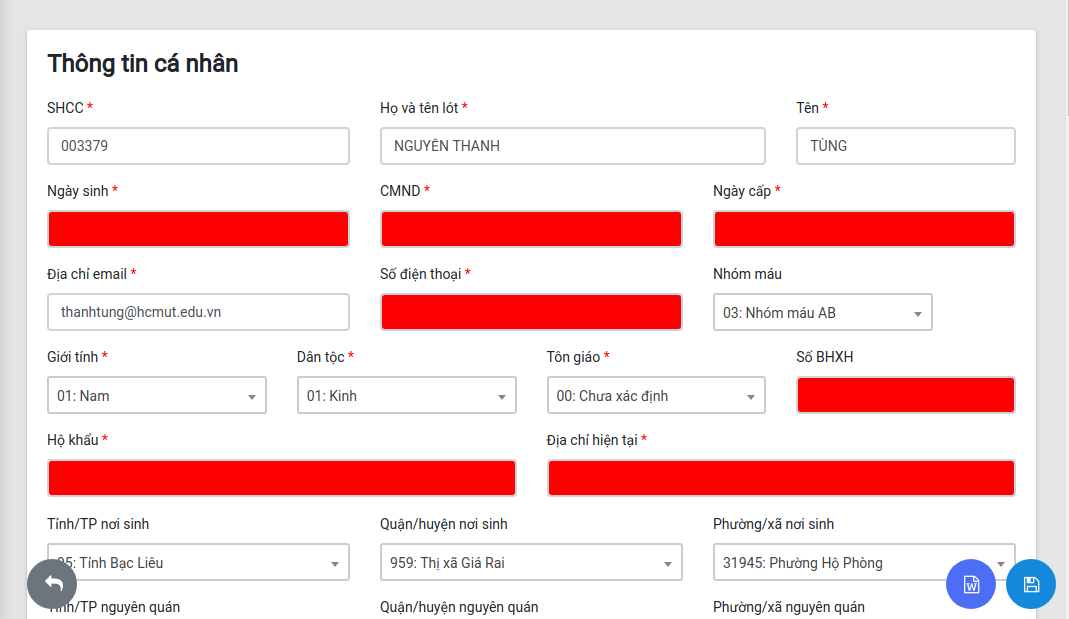
\includegraphics[width=15cm]{img/Screen/editthongtin.png}
  \captionof{figure}{Xem, chỉnh sửa thông tin cán bộ}
\end{center}
\subsubsection{Chức năng: Quản lý đối với một quá trình nghiệp vụ}
\begin{center}
  \captionsetup{type=figure}
  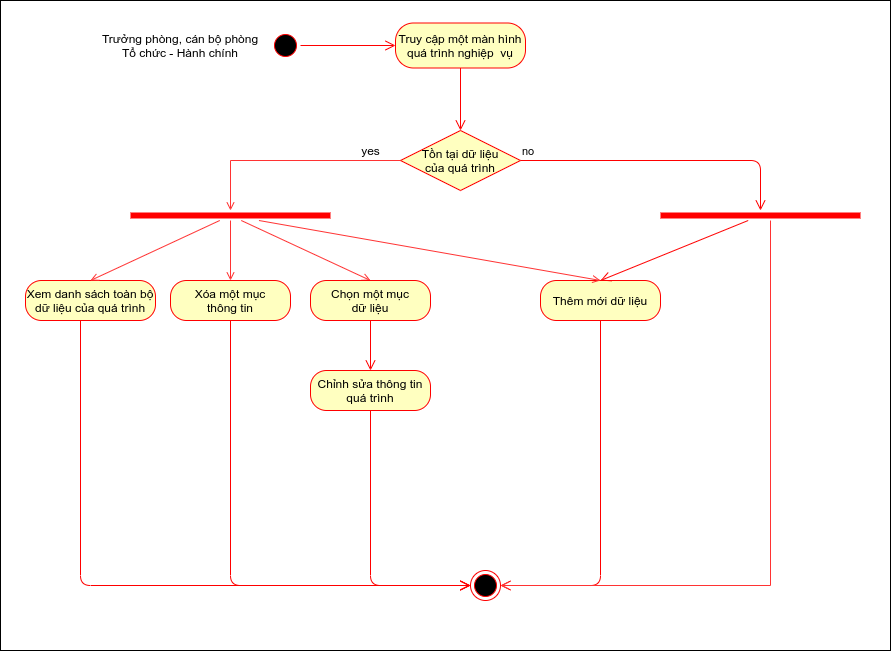
\includegraphics[width=15cm]{img/UML/TchcStaff/activityQuanLyQT.png}
  \captionof{figure}{Lược đồ Activity quản lý quá trình nghiệp vụ}
\end{center}

Chức năng này cho phép cán bộ phòng Tổ chức - Hành chính quản lý các quá trình nghiệp vụ của cán bộ trong trường. Cán bộ có thể thêm mới, chỉnh sửa hoặc xóa thông tin một quá trình. Ngoài ra, có thể tải toàn thông tin của quá trình dưới dạng tệp Excel.\\
\begin{center}
  \captionsetup{type=figure}
  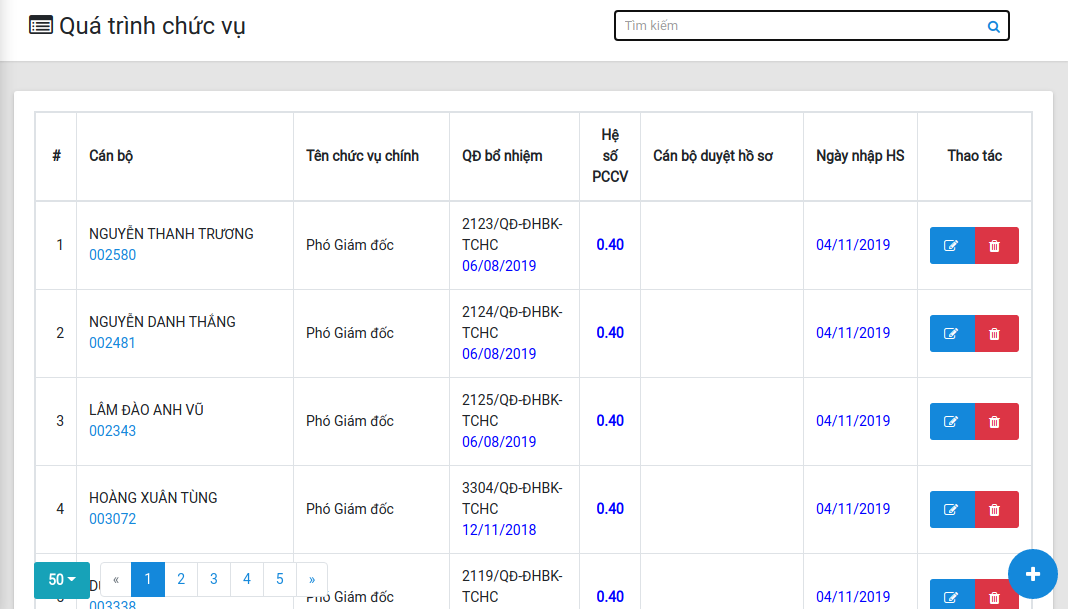
\includegraphics[width=15cm]{img/Screen/qlquatrinh.png}
  \captionof{figure}{Quản lý quá trình chức vụ của cán bộ}
\end{center}
\subsubsection{Chức năng: Quản lý các yêu cầu của cán bộ}
\begin{center}
  \captionsetup{type=figure}
  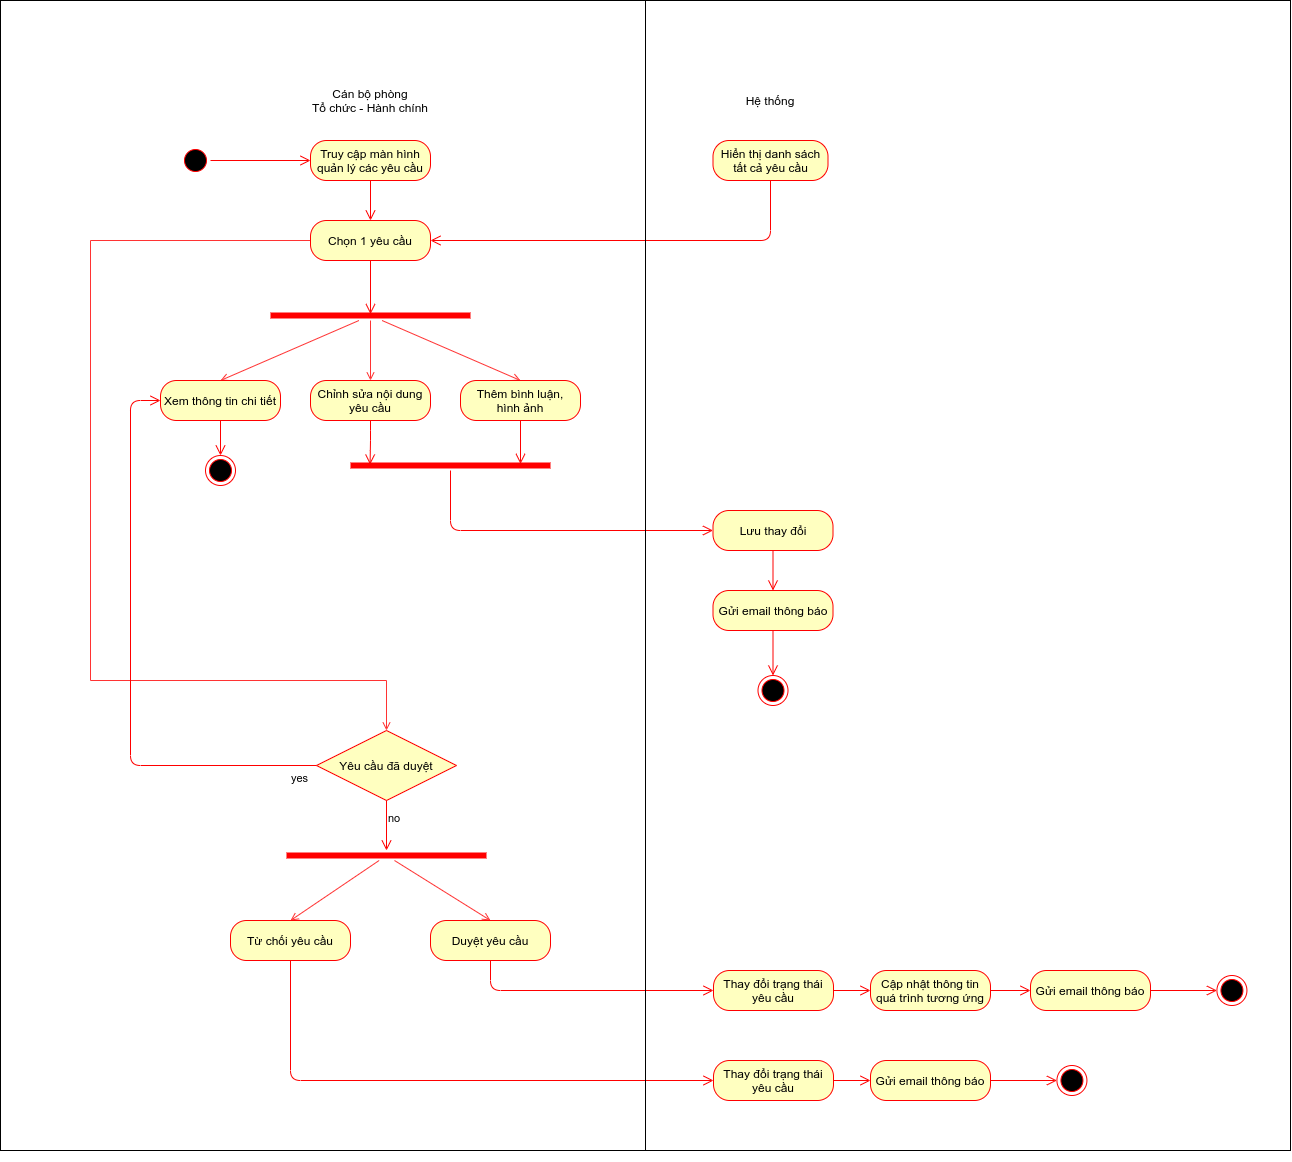
\includegraphics[width=15cm]{img/UML/TchcStaff/activityQLTask.png}
  \captionof{figure}{Lược đồ Activity cho chức năng quản lý các yêu cầu của người dùng}
\end{center}
\begin{center}
  \captionsetup{type=figure}
  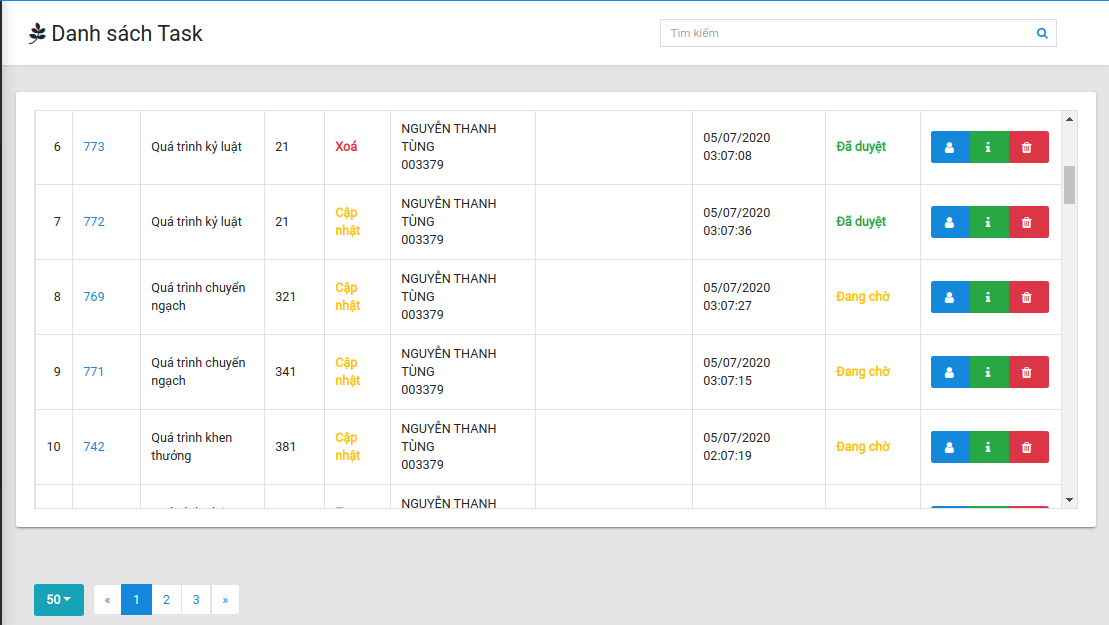
\includegraphics[width=15cm]{img/Screen/qltask.png}
  \captionof{figure}{Xem toàn bộ yêu cầu của cán bộ}
\end{center}

\begin{center}
  \captionsetup{type=figure}
  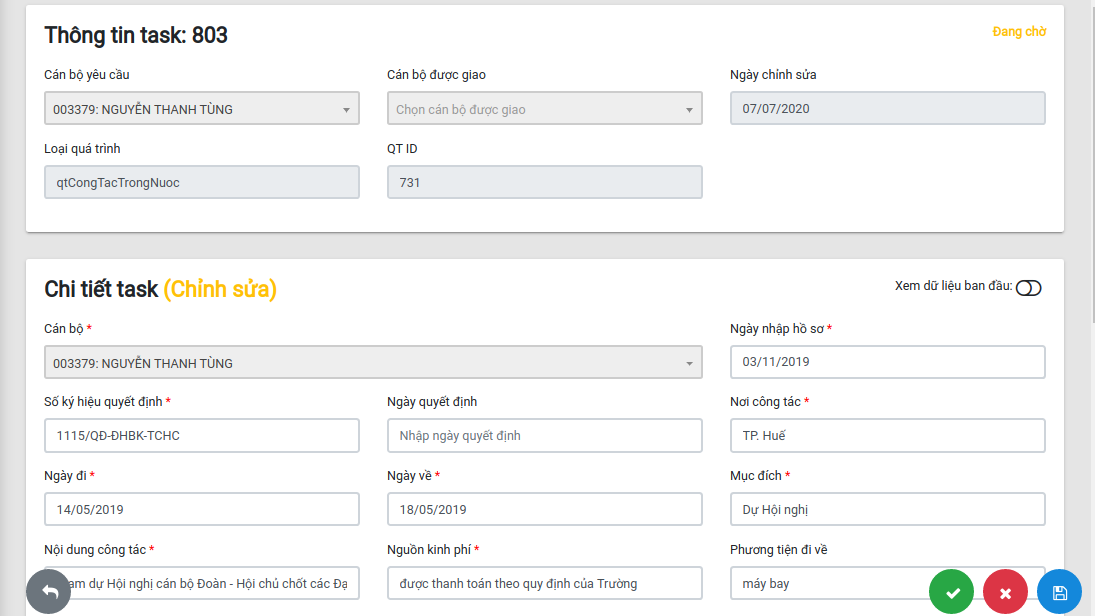
\includegraphics[width=15cm]{img/Screen/chitiettask.png}
  \captionof{figure}{Xem thông tin chi tiết yêu cầu của cán bộ}
\end{center}
Khi xem chi tiết yêu cầu, cán bộ phòng Tổ chức - Hành chính có thể chỉnh sửa thông tin mà người dùng yêu cầu, sau đó đồng ý hoặc từ chứ duyệt yêu cầu. Bên cạnh đó cán bộ có thể để lại bình luận kèm theo những hình ảnh mình chứng (nếu có) cho yêu cầu.\\
\subsection{Đối tượng: Cán bộ, công nhân viên của nhà trường}
\subsubsection{Chức năng: Quản lý thông tin}
\begin{center}
  \captionsetup{type=figure}
  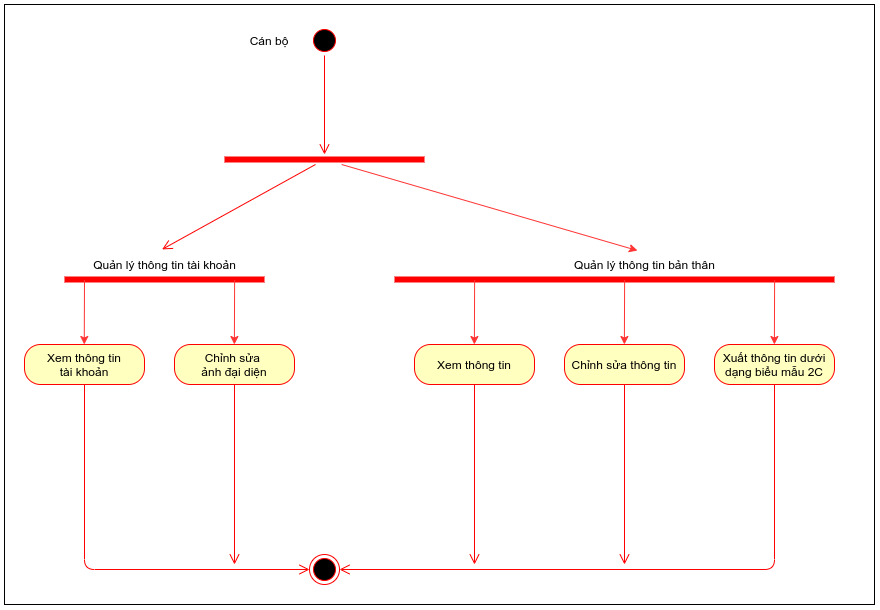
\includegraphics[width=15cm]{img/UML/User/activityQLThongTin.png}
  \captionof{figure}{Lược đồ Activity cho chức năng quản lý thông tin cho cán bộ}
\end{center}
\subsubsection{Chức năng: Quản lý quá trình}
\begin{center}
  \captionsetup{type=figure}
  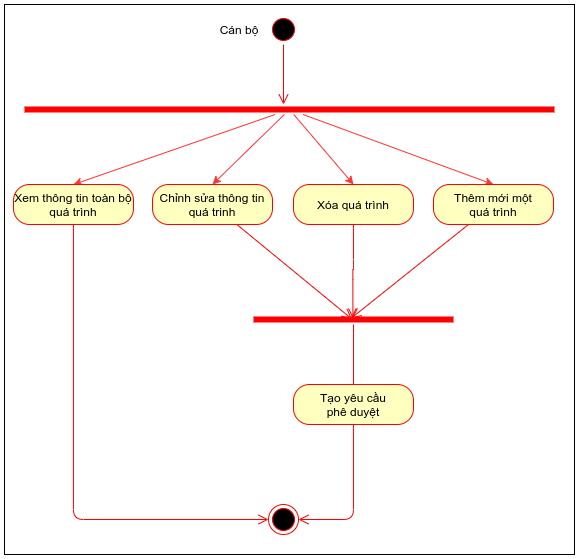
\includegraphics[width=15cm]{img/UML/User/activityQuanLyQT.png}
  \captionof{figure}{Lược đồ Activity cho chức năng quản lý quá trình cho cán bộ}
\end{center}

\subsubsection{Chức năng: Quản lý yêu cầu}
\begin{center}
  \captionsetup{type=figure}
  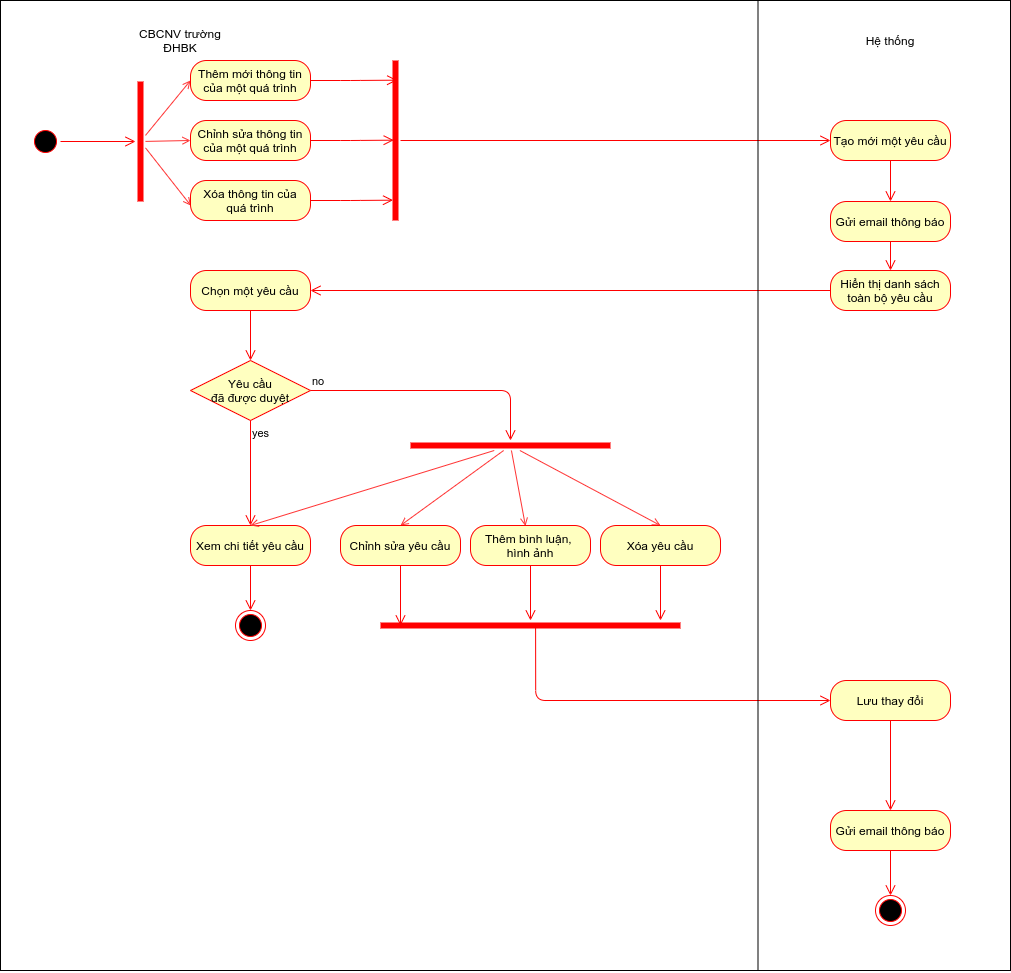
\includegraphics[width=15cm]{img/UML/User/activityQLTask.png}
  \captionof{figure}{Lược đồ Activity cho chức năng quản lý yêu cầu của cán bộ}
\end{center}